% Options for packages loaded elsewhere
\PassOptionsToPackage{unicode}{hyperref}
\PassOptionsToPackage{hyphens}{url}
\PassOptionsToPackage{dvipsnames,svgnames,x11names}{xcolor}
%
\documentclass[
  10pt,
]{article}
\usepackage{amsmath,amssymb}
\usepackage{iftex}
\ifPDFTeX
  \usepackage[T1]{fontenc}
  \usepackage[utf8]{inputenc}
  \usepackage{textcomp} % provide euro and other symbols
\else % if luatex or xetex
  \usepackage{unicode-math} % this also loads fontspec
  \defaultfontfeatures{Scale=MatchLowercase}
  \defaultfontfeatures[\rmfamily]{Ligatures=TeX,Scale=1}
\fi
\usepackage{lmodern}
\ifPDFTeX\else
  % xetex/luatex font selection
  \setmainfont[]{DejaVu Serif}
  \setsansfont[]{DejaVu Sans}
  \setmonofont[]{DejaVu Sans Mono}
\fi
% Use upquote if available, for straight quotes in verbatim environments
\IfFileExists{upquote.sty}{\usepackage{upquote}}{}
\IfFileExists{microtype.sty}{% use microtype if available
  \usepackage[]{microtype}
  \UseMicrotypeSet[protrusion]{basicmath} % disable protrusion for tt fonts
}{}
\makeatletter
\@ifundefined{KOMAClassName}{% if non-KOMA class
  \IfFileExists{parskip.sty}{%
    \usepackage{parskip}
  }{% else
    \setlength{\parindent}{0pt}
    \setlength{\parskip}{6pt plus 2pt minus 1pt}}
}{% if KOMA class
  \KOMAoptions{parskip=half}}
\makeatother
\usepackage{xcolor}
\usepackage[margin=18mm]{geometry}
\usepackage{longtable,booktabs,array}
\usepackage{calc} % for calculating minipage widths
% Correct order of tables after \paragraph or \subparagraph
\usepackage{etoolbox}
\makeatletter
\patchcmd\longtable{\par}{\if@noskipsec\mbox{}\fi\par}{}{}
\makeatother
% Allow footnotes in longtable head/foot
\IfFileExists{footnotehyper.sty}{\usepackage{footnotehyper}}{\usepackage{footnote}}
\makesavenoteenv{longtable}
\usepackage{graphicx}
\makeatletter
\def\maxwidth{\ifdim\Gin@nat@width>\linewidth\linewidth\else\Gin@nat@width\fi}
\def\maxheight{\ifdim\Gin@nat@height>\textheight\textheight\else\Gin@nat@height\fi}
\makeatother
% Scale images if necessary, so that they will not overflow the page
% margins by default, and it is still possible to overwrite the defaults
% using explicit options in \includegraphics[width, height, ...]{}
\setkeys{Gin}{width=\maxwidth,height=\maxheight,keepaspectratio}
% Set default figure placement to htbp
\makeatletter
\def\fps@figure{htbp}
\makeatother
\setlength{\emergencystretch}{3em} % prevent overfull lines
\providecommand{\tightlist}{%
  \setlength{\itemsep}{0pt}\setlength{\parskip}{0pt}}
\setcounter{secnumdepth}{-\maxdimen} % remove section numbering
\ifLuaTeX
  \usepackage{selnolig}  % disable illegal ligatures
\fi
\usepackage{bookmark}
\IfFileExists{xurl.sty}{\usepackage{xurl}}{} % add URL line breaks if available
\urlstyle{same}
\hypersetup{
  colorlinks=true,
  linkcolor={Maroon},
  filecolor={Maroon},
  citecolor={Blue},
  urlcolor={blue},
  pdfcreator={LaTeX via pandoc}}

\author{}
\date{}

\begin{document}

\section{Classical ECDLP experiment
programme}\label{classical-ecdlp-experiment-programme}

25 October 2026. Prospective designs, mathematical controls and
implementation checks; \textbf{no admitted scientific trials or attack
advantage}. This follows \href{../PLAN.md}{the research plan}. Classical
CPU/GPU algorithms only. Factor-base relation collection, index
calculus, quantum algorithms and quantum simulation are outside this
programme.

\subsection{Coverage and purpose}\label{coverage-and-purpose}

Cover the direct tagged-response proposal and all nine classical lead
families named in the plan. \url{LEADS.md} gives a separate card for
each family. This is exhaustive coverage of that named list, not of the
literature, every repository branch, or all possible algorithms. An
experiment can exhaust a finite, frozen search grammar; it cannot
exhaust an unspecified mathematical idea.

The desired research outcome remains a constructive, previously untested
EC-specific algorithm. Its novelty and complexity are unverified.
Collecting reproducible ordinary, unusual, negative or inconclusive
observations is also a valid study outcome. Correct execution,
mathematical falsification and competitive performance are separate
questions.

Several originals, including IDEA-050, IDEA-111, IDEA-156 and IDEA-379,
were formulated for factor-base/index-calculus pipelines. Their original
pipelines are excluded. Their cards describe explicitly different
direct-inversion successors whose missing constructions remain visible.
A proved obstruction is a control to reproduce and respect; it is not a
reason to rerun the same algorithm under a new name.

\subsection{Outcome vocabulary}\label{outcome-vocabulary}

Each trial reports one execution outcome: \texttt{complete\_valid},
\texttt{wrong\_output}, \texttt{timeout}, \texttt{memory\_limit},
\texttt{invalid\_input}, \texttt{infrastructure\_error}, or
\texttt{not\_executable}. Preserve every attempt, including failed
searches and constructor failures. A counterexample falsifies its exact
universal identity; a timeout does not. No outcome automatically changes
an official lead or hypothesis status.

Distinguish five research milestones:

\begin{enumerate}
\def\labelenumi{\arabic{enumi}.}
\tightlist
\item
  \textbf{Encoding correctness:} exact agreement with an independent
  reference, including exceptional cases and unique witnesses. This
  qualifies the instrument only.
\item
  \textbf{Observation:} a frozen statistic with its inputs, reference,
  uncertainty and all outcomes. An anomaly is unnecessary.
\item
  \textbf{Mechanism correctness:} an explicit public constructor, an
  identity or invariant with exact domain, and closure under
  composition. One counterexample rejects that version.
\item
  \textbf{Scoped performance:} measured complete costs against matched
  baselines. A local reduction is labeled local; it is not a solver
  gain.
\item
  \textbf{Novel algorithm or asymptotic claim:} additionally requires
  prior-art collision review, independent reconstruction, a uniform
  algorithm and a justified time/memory analysis. A short size ladder
  cannot establish an exponent.
\end{enumerate}

\subsection{Shared input and blinding
contract}\label{shared-input-and-blinding-contract}

\textbf{Development fixtures already implemented} are listed in
\url{CHECKS.md}. They are tiny synthetic unit-test inputs, not the
registered scientific cohort below.

\textbf{Prospective discovery cohort:} subgroup bit lengths 8, 10 and
12; four curves per length; exhaustive canonical scalars.
\textbf{Prospective confirmation cohort:} six fresh curves at each of
12, 14, 16 and 18 bits, eight independently drawn uniform scalars per
curve: 24 curves and 192 random targets. Keep the forced scalars 0, 1
and r−1 and exceptional arithmetic cases in a separate correctness
suite; do not replace random performance targets with them. The two
cohorts have disjoint curve IDs and generator domains. These exact
scientific inputs have not yet been generated or registered.

Before admission, register each (p,a,b,\#E,r,h,P), canonical point
encoding, subgroup and field certificates, curve-family stratum,
generation seed/algorithm, rejection history and content digest. For
these sizes, exact point enumeration can certify \#E, trial division can
certify primality, and {[}r{]}P=O with P≠O certifies the prime subgroup
order. Check nonsingularity, odd p, r prime, r≠p, \#E≠p and exact
cofactor h=\#E/r. Specify the public registry authority; do not silently
invent canonical IDs.

Freeze a deterministic hash-stream rejection sampler and its
accepted/rejected records, rather than choosing curves after inspecting
results. The main stratum is ordinary non-anomalous curves with j
different from 0 and 1728; special-j, special-prime, supersingular or
extension-field families require separately registered strata and
matched baselines. Describe the induced sampling distribution; it is not
uniform over all elliptic curves. Include a nontrivial-cofactor fixture
and targets outside the subgroup as rejection/zero-response controls.

Freeze and publish the constructor, compiler options, grammar,
elimination schedule policy, stopping rule and input-manifest hashes
before opening confirmation targets. An input custodian generates
synthetic public Q values and keeps k, scalar-derived filenames and
reverse lookup tables outside the candidate process. An output checker
alone uses the truth. Record custody and process access. A public seed
that reconstructs k is not a blind target. If isolation is unavailable,
call the test non-blind. A new method version gets a fresh confirmation
cohort; do not retune on its held-out results.

Curves are the replication units. Eight targets on one curve share setup
and arithmetic and are not eight independent curves. Report per-curve
summaries and every target. Use a curve-cluster bootstrap for
descriptive uncertainty in paired cost ratios; with six curves per size,
call uncertainty coarse. These counts are an initial diagnostic
allocation, not a power calculation for a particular conjecture.
Rare-event hypotheses require a separately frozen sample-size
calculation from their predicted probability.

\subsection{Direct response: an executable specification and four
tests}\label{direct-response-an-executable-specification-and-four-tests}

For canonical 0≤b\textless r, total scalar multiplication C(b) and
target Q, use

\[R=\mathbb F_2[\varepsilon_0,\ldots,\varepsilon_{\ell-1}]/(\varepsilon_i\varepsilon_j\text{ for all }i,j),\qquad
Z_Q=\sum_b [C(b)=Q]\left(1+\sum_j b_j\varepsilon_j\right).\]

For Q={[}k{]}P there is one accepted scalar and Z\_Q=(1,k). A
square-zero ring element is an ordinary pair (constant bit, tag
bit-vector); addition is XOR and (a,u)(b,v)=(ab,av+bu). This is known
algebraic model counting. Enumerating all b costs O(r) scalar
evaluations and is a reference, never the proposed speedup.

\textbf{D0 --- instrument checks.} Enumerate all bit inputs, including
b≥r, all subgroup targets and selected outside targets on fixed tiny
fixtures. Compare independently coded affine and Jacobian arithmetic,
enumerate exceptional additions, and count satisfying transition
witnesses. Inject one unconstrained Boolean auxiliary variable and
verify that two identical witnesses cancel in characteristic two. Inject
an intentionally wrong rewrite and ensure the checker returns a boundary
counterexample. Check tagged coefficients, not just ordinary parity.
Pass: zero mismatches in the declared finite suite and successful
detection of each injected defect. Failure: a concrete mismatch
invalidates that encoding/checker version. Limits: point-level
deterministic arithmetic is not a gate-level Boolean circuit or a
carry/wire proof.

\textbf{D1 --- exact micro-block discovery.} First construct total,
gate-level one- and two-step double-and-add blocks, b\textless r and
canonical-output constraints. Fix wire layout, finite rewrite grammar,
coefficient domain and an exact boundary enumeration before search.
Candidate output must name the original block, replacement, target pins,
every retained boundary bit and construction cost. Compare reference
contraction to replacement for every boundary assignment on registered
tiny instances, then overlapping two-block compositions. Require
equality of all coefficients or a proved narrower invariant closed under
composition. Generic XOR elimination, Boolean simplification and
ordinary fixed-window merging are controls. Preserve every rejected
candidate and its first counterexample. A finite grammar can be
exhausted only after its file and bounds are frozen; that file and a
gate compiler are currently missing.

For a compiled-counting adapter, test decomposable conjunctions,
deterministic disjunctions and smoothing explicitly. Positive and
negative scalar-literal weights sum to epsilon\_j, not to 1. Omitting an
unused scalar variable therefore changes the tagged count unless its
actual weight sum is included. Verify the chosen compiler's theorem and
coefficient-domain assumptions rather than substituting ring operations
into an arbitrary Boolean DAG.

\textbf{D2 --- structure and construction measurement.} For each
surviving rule measure constraints eliminated, maximum
participating-index union, peak live entries, encoded coefficient bits,
constructor operations, rule applications and total checking/recovery
work. Run the same generic simplifier on the EC block, an injective
affine-bit-map control and a tiny explicit random-permutation control.
Charge permutation table generation/storage. Arithmetic-mutated controls
must retain total unique-extension semantics and disclose their encoding
differences. An invertible basis change alone preserves the original
function and is not a destroyed-structure null. Record whether any
difference is specifically attributable to the EC identity. A small
answer, separator, numerical rank or expression is insufficient if its
construction is expensive.

The fixed-window matrix control in \url{window-control.md} has scalar
rank r−1 over F₂. It explains why a dense global point-state low-rank
replacement cannot be presumed. It does not prohibit a different
bit-level, nonlinear or target-conditioned algorithm. No gate-level
discovery or D2 comparison has run.

\textbf{D3 --- frozen complete solver.} Admit only after there is an
actual constructor and composition argument. Run every random
confirmation target and the separate correctness suite. Recover k using
public inputs alone and verify {[}k{]}P=Q independently. Charge failed
branches, compilation, schedule search, target specialization,
contraction, candidate extraction and verification. Compare a cold
first-target run with matched rho, relevant automorphisms, BSGS where
memory permits, and the strongest available exact compiler on the
identical problem. If a comparator is unavailable, state that limitation
and do not claim superiority to it. A generic integer \#SAT result is
not automatically a characteristic-two tagged count; bind and verify the
adapter.

For an exploratory local-gain screen, a twofold reduction in the
declared dominant local operation on two registered sizes warrants a
fresh composition/cost test. That threshold is an engineering choice,
not a theorem or a publication rule. For a complete-solver performance
study, freeze its minimum effect and paired estimator only after
baseline calibration; include A/A repeatability first. No performance
threshold is retrofitted to results.

\subsection{Baselines, costs and
statistics}\label{baselines-costs-and-statistics}

Use identical public Q values, curve strata, arithmetic backend,
threads, compiler, hardware placement and stopping/correctness policy.
Freeze baseline tuning on development inputs. Rho uses negation and
applicable automorphisms with cycle handling; credit known endomorphism
speedups to both sides where applicable. A BSGS comparator gets its
actual storage budget. Record baseline seeds and stochastic spread; do
not compare a lucky candidate run with a single unlucky walk.

Use A/A repetitions to expose slot/host drift, randomize
candidate/baseline execution order and record process placement and
frequency/thermal conditions when available. Wall time, CPU time, field
additions/multiplications/inversions, bit operations and
allocation/storage bytes have distinct units. Raw XOR counts are not
directly comparable to group additions. A full-cost elapsed-time claim
needs controlled calibration and placement. Preserve compilation cost
and circuit-size/width counters even when timing noise dominates.

Primary per-target cost is cold setup + preprocessing + target work +
failed attempts + recovery + verification; record peak live and
persistent memory separately. Secondary many-target costs must name the
reuse count m and report (setup+sum target costs)/m. Compare with
preprocessing baselines for the same m. Do not hide an O(r) truth table
in setup. Preserve censored/time-limited targets, success fraction and
resources consumed; successful-only averages are prohibited.

Report descriptive distributions and paired per-curve ratios. Any
exploratory size fit states its model, range, confidence and dependence
assumptions; it cannot establish an asymptotic exponent. Confirmation of
a new speed/attack-cost claim requires repository progress-fidelity
records and an independent session, neither supplied by this design
document or its assisting agents.

\subsection{Frozen receipt and machine
protection}\label{frozen-receipt-and-machine-protection}

Every scientific run needs immutable code/commit and dirty state, input
and protocol hashes, exact argv, compiler/build identity, host/resource
identity, UTC times, seeds, outcome, raw counters with units,
output/certificate hashes, checker identity and all stdout/stderr.
Record requested/completed/failed/censored counts by arm. Archive a
failure before retrying; link the new attempt. Large artifacts follow
the shared object-store policy, with hashes and readback; do not
silently drop data to fit Git limits.

Use one worker initially and an explicit RAM limit below the host
allocation. Set a process watchdog from the declared worst-case input
and a resource estimate during admission. These protect the host and
classify censoring; they are not lifetime research budgets or evidence
of impossibility. The programme has no arbitrary campaign spending cap.
Fixed cohorts end their registered test; subsequent work uses an
additive new protocol.

\subsection{Readiness and next
actions}\label{readiness-and-next-actions}

The repository requires a prospective runnable specification, launcher,
committed input/source hashes, executor handoff/queue and lawful lane
before approval. Its read-only \texttt{experiment\_preapproval.py} must
return \texttt{approvable:\ true}; after the committed approval/archive,
the selector must return \texttt{execution\_state:\ ready} before
scientific dispatch. No such receipt is fabricated here. Development
self-tests below exercise code, not those admission gates.

Immediate work completed: per-lead designs, a point-level C++ reference,
finite correctness checks and a scoped window-control derivation.
Immediate implementation debt: registered scientific cohorts; a
bit-level total circuit and unique-wire checker; exact finite grammar;
lead-specific constructors and adapters; complete
launch/admission/custody records. See \url{READINESS.json} and the
\href{../../../../problems/direct-ecdlp-cancellation-construction.md}{named
obstruction}.

Prioritize D0 instrument completion and D1 exact blocks. In parallel,
reproduce the lossy-panel finite references and deterministic rigidity
proof as controls, and test only explicitly supplied
EDS/endomorphism/automaton constructions. Do not run undefined
coefficient, inverse-state or Pfaffian oracles. New direct successors of
blocked originals get fresh identities rather than rewriting frozen
evidence. Revisit a scoped negative only when its stated assumption
changes or a specific missing constructor appears.

This programme changes no canonical frontier or official scientific
disposition. It provides a concrete path to distinguish a correct
instrument, informative observation, failed construction, resource
limit, local identity and complete classical algorithm.

\newpage

\begin{figure}
\centering
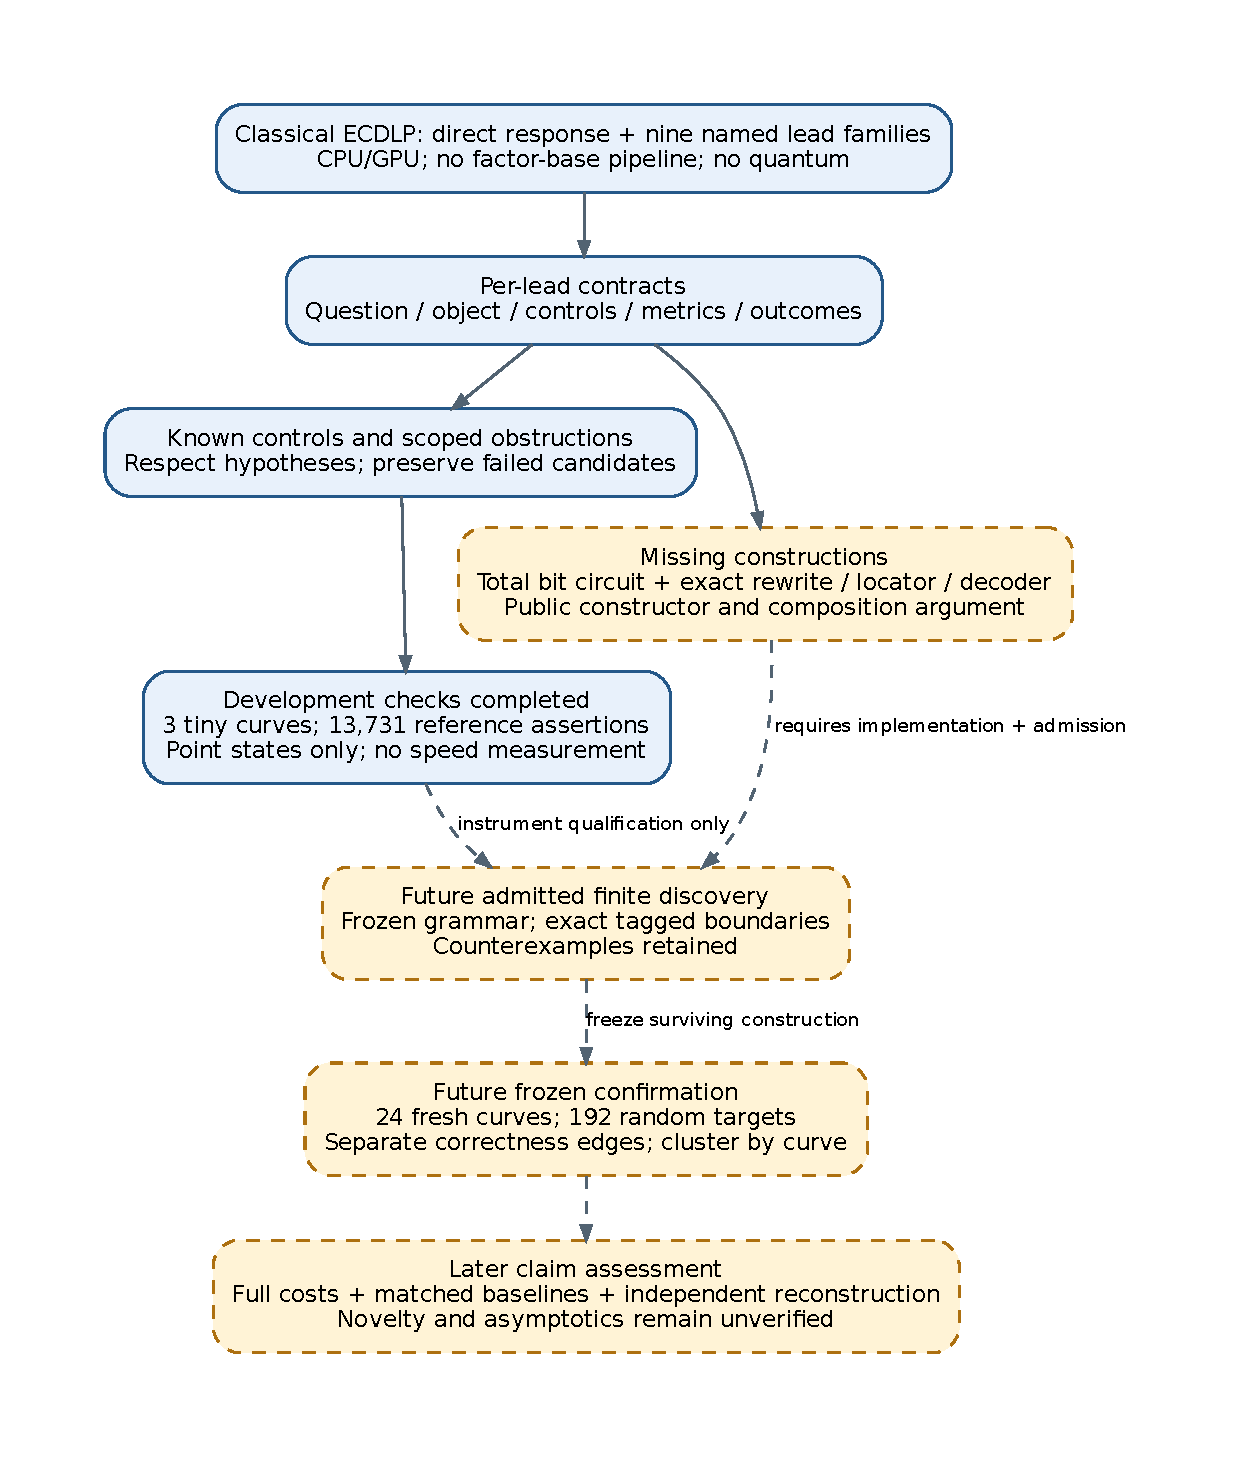
\includegraphics[width=0.78\textwidth,height=\textheight]{programme.pdf}
\caption{Completed development scaffolding and proposed scientific
stages. Dashed amber boxes are pending; no measured speedup is
depicted.}
\end{figure}

\newpage

\section{Experimental cards for the nine cited classical lead
families}\label{experimental-cards-for-the-nine-cited-classical-lead-families}

Design date: 2026-10-25. These are proposed protocols, not approved
experiment records, executed trials, or scientific dispositions. They
exhaust the nine named prior-family rows in the companion plan, not
classical ECDLP research. The direct tagged-count workstream has its own
card. No card authorizes quantum computation or index calculus.

\subsection{Common design and outcome
vocabulary}\label{common-design-and-outcome-vocabulary}

Use public synthetic non-anomalous odd-prime-field instances with a
certified odd-prime subgroup order \texttt{r}. Register the companion
programme's proposed discovery fixtures before scientific admission:
four curves at each of 8, 10 and 12 subgroup bits. All canonical scalars
are the discovery truth set; a truth process may enumerate them, but its
tables and labels are not candidate inputs. Freeze the algorithm,
feature definitions, rational/finite-field coefficient domain,
exceptions, seeds, and exact manifest before fresh tests. A candidate
that survives discovery uses the companion held-out allocation of six
fresh curves at each of 12, 14, 16 and 18 bits and eight targets per
curve. This is a contingent allocation, not existing fixtures or an
asymptotic argument. Special automorphism families are separate strata
with matched baselines.

Every run records exact successes, misses, false outputs,
multiplicities, undefined cases, operation counts, setup, discarded
trials, peak live storage, serialized state/coefficient sizes, and
verification. All cold construction costs count. Discovery enumeration
is instrumentation, not a solver speedup. A theorem-only card records a
proof obligation rather than running a benchmark with an assumed oracle.
Resource limits censor trials; they do not refute mathematics.

Three different outcomes must be retained: \textbf{measurement success}
means the declared observations were obtained and controls passed;
\textbf{candidate failure} means an exact claimed property has a
counterexample or a measured cost objective failed at the tested scope;
\textbf{inconclusive/impeded} means missing construction, inadequate
resolution, failed controls, or infrastructure. Ordinary behavior and
null observations are complete useful measurements. A mechanism signal
or stage gain is separate from a whole-solver gain. No empirical fit on
this ladder proves an exponent below one half.

Each candidate implementation gets a collision paragraph against its
cited record and the generic tool that already performs the operation.
Published interpretation requires independent checking under the
repository contract. These cards do not reopen retired hypotheses or
modify frozen gates.

\subsection{L1. Prime-to-p lifts and non-homomorphic local
sections}\label{l1.-prime-to-p-lifts-and-non-homomorphic-local-sections}

\textbf{Prior boundary.} \texttt{LEAD-EXO-padic-jet-canonical-lift}
records the prime-to-characteristic additive-log obstruction and
previous hard-lift versus computable-section tests. An additive
homomorphism from an order-\texttt{r} group into a p-primary additive
target is zero when \texttt{r\ !=\ p}. That scoped theorem needs no
performance rerun. A hard lift defined as \texttt{{[}k{]}S(P)} already
contains the unknown scalar. The potentially testable successor is a
specified, cheap, non-homomorphic section; it does not inherit additive
linearity.

\textbf{Concrete diagnostic.} For a nonsingular integral lift of
\texttt{E} modulo \texttt{p\^{}2}, freeze \texttt{A,B} and an explicit
point section \texttt{S}. One reproducible candidate chooses the
Teichmuller lift of the canonical x-coordinate and Hensel-lifts the
observed y-coordinate; handle infinity separately. For an odd-order
subgroup, a nonidentity rational point has \texttt{y\ !=\ 0}, so the y
derivative is a unit. Compute
\texttt{D\_S(R)\ =\ t({[}r{]}S(R))/p\ mod\ p}, with \texttt{t=-x/y} at
infinity using a correct projective implementation. Record the defect
\texttt{D\_S(U+V)-D\_S(U)-D\_S(V)} and the entire canonical-scalar
profile \texttt{D\_S({[}k{]}P)}. These are computable from public points
without k. Other section families must be declared separately before
measurements; do not silently tune a section after observing labels.

\textbf{Measurements and controls.} On discovery curves enumerate all k
and all pairs on the smallest four curves; use a fixed 65,536-pair
sample on the remaining curves if exact pair enumeration is not selected
in the frozen plan. Positive controls are the genuinely additive
formal-group law and a known anomalous-curve control kept outside the
target population. A deliberately hard lift \texttt{{[}k{]}S(P)} is a
labeled leakage trap whose linearity is expected, not an attack. Compare
the same fixed scalar predictor and profile statistics with 99
permutations of scalar labels preserving the feature multiset. Record
the sign symmetry and identity separately. Report the exact chance
reference induced by each permutation scheme rather than asserting a
universal \texttt{1/p} accuracy.

\textbf{Advance criterion.} A new section has a reproduced
public-computable relation or frozen predictor whose held-out deviation
survives controls; report its effect and uncertainty before interpreting
it. Exact scalar recovery then requires an explicit decoder, complete
candidate list, and charged costs. \textbf{Failure:} one counterexample
rejects claimed exact additivity; hard-lift advice rejects the claimed
public constructor. Matching null labels is a scoped observational null,
not closure of every section. \textbf{Impeded:} no explicit section,
insufficient test resolution, or undefined exceptional lifts. The next
mathematical question after a signal is why the section defect preserves
scalar information across unseen curves and wraparound.

\subsection{L2. Elliptic nets / EDS and target-specific nonlinear
locators}\label{l2.-elliptic-nets-eds-and-target-specific-nonlinear-locators}

\textbf{Prior boundary.} \texttt{LEAD-EXO-elliptic-net-eds} and IDEA-006
already cover short linear annihilators, translated coordinate blocks,
ordinary displacement-rank tautologies, and the old Somos sieve.
Repeating that sieve is outside this programme because it is a
relation-collection route. Net recurrences do not supply an index
inverse. The source itself leaves target-specific nonlinear locators and
an unexplained rank-two-net null asymmetry open; obtain the raw prior
evidence before treating that asymmetry as a fresh observation.

\textbf{Runnable diagnostic.} Freeze exact division-polynomial/net
recurrences with normalization and zero handling, and build (i)
known-index net values and (ii) target-translated public coordinate
blocks \texttt{a\_Q(n)=x(Q+{[}n{]}P)} with a distinct infinity symbol.
Verify every recurrence on discovery truth, including zeros. Measure
minimal linear complexity of every prefix of lengths \texttt{8,16,...}
up to the available period, both point signs, and nonlinear-predictor
residuals for a frozen finite grammar. A permissible exploratory grammar
is quadratic polynomials in a four-value coordinate window, fitted on
disjoint windows and tested on all untouched windows;
rank/identifiability and coefficient-storage costs are reported. This
measures prediction, not scalar location. Arithmetic domains and
infinity charts must be explicit.

For that finite quadratic grammar there are exactly 15 monomials of
degree at most two in four variables. Fit a deterministic linear system
for \texttt{a(n+4)} over \texttt{F\_p}; freeze lexicographic monomial
order and a canonical free-variable assignment. Use the first half of
finite-chart windows for fitting and the second half for testing, and
report all infinity-crossing windows separately. Excluding a window is
permitted for this declared chart diagnostic only; a solver still has to
handle it. A second grammar is a separate registered search, not silent
post-hoc tuning.

\textbf{Controls.} Same-normalization known EDS identities; matched
random periodic sequences; random scalar relabeling of the exact same
coordinate/net-value multiset; Berlekamp-Massey and the existing
recurrence as predictor controls. A hidden scalar shift in the training
labels is a leakage trap. A low-degree recurrence that predicts values
while leaving all cyclic orientations feasible is recorded as such.

\textbf{Constructor gate.} Before any direct-recovery benchmark, supply
an explicit locator whose coefficients/representation are constructed
from \texttt{(E,P,Q)} and whose roots or reverse path yield the
canonical k, with a charged uniform construction and complete ambiguity
list. Name the algebraic identity beyond the already-known recurrence. A
sparse expression naming an unknown index is not a constructor.
\textbf{Success:} exact recurrence/locator measurements with all
controls; a useful candidate additionally reduces orientation ambiguity
on fresh targets with charged total cost. \textbf{Failure:} one false
locator root/missed scalar rejects exactness; linear complexity above a
claimed bound rejects that bound on its declared family. \textbf{Null:}
frozen nonlinear prediction matches its controls. \textbf{Impeded:} the
nonlinear locator has not been supplied. No finite predictor panel
closes all nonlinear locators.

\subsection{L3. Endomorphism actions and coordinate
observables}\label{l3.-endomorphism-actions-and-coordinate-observables}

\textbf{Prior boundary.} \texttt{LEAD-STR-endo-scalar-action-generic}
covers group-element oracles with known eigenvalues: on the prime-order
subgroup, \texttt{phi\_i(R)={[}lambda\_i{]}R}, so
\texttt{phi\_i(Q)={[}k{]}phi\_i(P)} is the same unknown congruence. It
does not rule out every computation on actual field-coordinate bits.
Known constant-factor automorphism gains remain legitimate matched
controls.

\textbf{Exact control experiment.} In each declared automorphism
stratum, verify \texttt{phi\_i(P)={[}lambda\_i{]}P} and
\texttt{phi\_i({[}k{]}P)={[}lambda\_i\ k{]}P} for every discovery k. For
every proposed short witness-lattice vector c, classify the certificate:
\texttt{sum\ c\_i\ lambda\_i\ =\ 0\ mod\ r} is k-independent, while any
claimed scalar constraint must be written explicitly and checked against
all k. The \texttt{j=0} relation \texttt{1+lambda+lambda\^{}2=0} is a
deliberate positive trap: a short vector satisfying it cannot recover k.
Compare any generic walk with the same walk using the same automorphism
quotient, not a baseline deprived of the quotient.

\textbf{Successor gate.} A new candidate must name an efficiently
computable field-valued or bit-valued observable and the exact operation
it supplies beyond group-image actions. Freeze its decoder and candidate
ambiguity before held-out tests. Do not accept an unimplemented
``coordinate oracle.'' \textbf{Success:} complete exact certificate
classification and measured constant-factor effects, or a separately
constructed coordinate operation that survives blind recovery.
\textbf{Failure:} k-independent vectors reject the claimed scalar
inference; scalar-indexed eigenvalue/orientation tables reject the
constructor. \textbf{Null:} no additional recovery beyond the matched
automorphism baseline at tested sizes. \textbf{Impeded:} no non-generic
observable/decoder has been constructed. The generic theorem is not a
blanket lower bound on coordinate algorithms.

\subsection{L4. Matchgate / Pfaffian transform, direct-inversion
successor to
IDEA-050}\label{l4.-matchgate-pfaffian-transform-direct-inversion-successor-to-idea-050}

\textbf{Scope correction.} IDEA-050's original hypothesis is explicitly
a factor-base relation/matrix/descent scheme and is outside this user's
scope. Do not run or relabel its original experiment as non-IC. This
card is a different, still-unconstructed direct-inversion successor:
transform the exact scalar-program factor network conditioned on Q.
Matchgate computation and basis transforms are established tools, not
the proposed novelty.

\textbf{Finite preflight.} Freeze one- and two-step total scalar blocks,
their boundary variables, equality/fan-out tensors and target pins.
Start over exact rational weights so matchgate signs and coefficient bit
growth are visible; do not transfer a characteristic-zero Pfaffian
theorem to characteristic two or the tag ring without a proof. Candidate
basis matrices must be explicit, invertible, public and constructed
without k. Evaluate all parity-support and matchgate/Grassmann-Pluecker
identities exactly on every local transformed signature. Include
membership/range/equality/exception tensors, not just a favorable
arithmetic gate. A basis-search grammar and its finite bounds must be
committed before search; every failed arm is retained.

One concrete first search grammar is a single common 2-by-2 rational
matrix M whose entries are in \texttt{\{-1,0,1\}}, excluding determinant
zero. Fix the index convention so one end of each contracted wire
transforms by M and the other by its inverse transpose; verify that
their contraction is unchanged. There are at most 81 arms before
singular matrices are removed. Check the identical M against every
required tensor of the frozen block. This very narrow grammar is
deliberately exhaustive within its declared bounds; failure says nothing
about all bases. Larger rational entries, per-wire bases, extension
fields or alternate planar realizations require separately frozen
successor grammars.

\textbf{Composition and controls.} Positive control: a known planar
matchgate network conjugated by an explicit invertible basis. Negative
control: random signatures with identical arity and declared support.
Mechanism control: untransformed exact contraction and the same generic
simplifier. For a surviving basis, construct the complete graph, account
for crossings/planarization and bit tags or repeated scalar-bit
conditioning, and verify the Pfaffian answer against direct contraction.
A valid local signature does not establish a planar tractable whole
network.

\textbf{Advance criterion.} Exhibit the basis, realizations, exact
identity checks, global graph construction, and a source-free recovery
procedure for every scalar bit. Charge basis discovery, rational
numerator/denominator growth, all conditioned Pfaffians, graph width,
zero cases and output verification. \textbf{Failure:} a violated exact
identity rejects that basis on that signature; missing
equality/crossing/exception realization rejects the asserted
whole-network reduction; one incorrect bit rejects recovery. A finite
unsuccessful basis search rejects only its grammar. \textbf{Impeded:} no
explicit basis/planar construction; this is the current direct
successor's status. A full arbitrary-basis impossibility claim would
need a separately proved invariant, not a numerical rank plot.

\subsection{L5. Radical ladder quotient, target-local successor to
IDEA-111}\label{l5.-radical-ladder-quotient-target-local-successor-to-idea-111}

\textbf{Scope correction and theorem gate.} IDEA-111 is theorem-deferred
and its original factor-base/descent path is out of scope. Its frozen
text explicitly requires independent review before solver execution.
Keep that gate and all original records unchanged. A direct target-local
functional is a different question, not an automatic escape from the
rank obstruction.

\textbf{First discriminating proof.} Write the exact complete finite
branch ideal, including selectors, field equations, range restriction,
exceptional components and quotient map. For a reduced finite algebra
over \texttt{F\_p} whose complete geometric support consists of m
distinct rational points, the coordinate-ring dimension is m by the
Chinese remainder theorem. A quotient algebra retaining a bijection to
all branch points therefore cannot have dimension below their count. If
all length-t branch labels remain recoverable, shared syntax does not
avoid this dimension/output obligation. Check whether the proposed
quotient genuinely changes those hypotheses, rather than measuring a
smaller input DAG.

\textbf{Only after its gate, finite diagnostic.} For approved symbolic
depths \texttt{t=1,...,6}, enumerate the exact valid path set for
reference and compare every decoded quotient point and multiplicity.
Record number of branches, radical normal-form dimension, coefficient
bits, construction cost and decoder cost. Include repeated-output
branches with distinct selector labels, zero denominators, infinity, and
both signs. Controls: duplicated identical components with a known
quotient; disjoint affine branches with direct-product coordinate ring;
the ordinary shared-prefix DAG. One lost or invented branch rejects
losslessness at that depth.

\textbf{Direct target-local question.} Once Q is pinned and canonical
range enforced, the valid scalar graph has one point, so its reduced
coordinate ring has dimension one. That is a correctness fact, not a
cheap constructor: computing its generator can already reveal k. A
successor must give a public target-conditioned invariant closed under
composition without constructing or decoding the full branch union.
Measure the full construction, specialization and recovery costs; share
this experiment with the direct tagged-count workstream rather than
counting it as independent evidence.

\textbf{Success:} a checked structural statement at its exact
quantifiers, then an explicit target-local construction and verified
compositional rule if one is found. \textbf{Failure:} a counterexample
to losslessness or the proposed dimension bound. \textbf{Null:} no
compression beyond the declared duplicate control in the tested depth
grammar. \textbf{Impeded:} missing theorem/independent review or missing
target-local constructor; do not launch an assumed quotient benchmark.

\subsection{L6. Reverse automata, successor conditions for rejected
IDEA-070}\label{l6.-reverse-automata-successor-conditions-for-rejected-idea-070}

\textbf{Prior boundary.} IDEA-070 is \texttt{rejected\_merged}, with no
active experiment gate. Small-state net/orbit descriptions and a missing
orientation map are occupied routes. For \texttt{r} near p, base-p
scalar notation has essentially one digit, so a putative shallow
automaton may hide r outgoing labels. A small minimal acceptor of a
single already-known target word is also vacuous: every single word has
a short acceptor if that word is supplied.

\textbf{Diagnostic without promotion.} Freeze a point-computable
observable, base (\texttt{p} for the original question; base 2 as a
separately named successor), digit order, canonical padding and output
alphabet. On the discovery truth sequence, construct the exact
bounded-depth residual functions and minimize only for measurement;
record all states, transitions, transition-label bits, output ambiguity,
constructor cost and number of scalars compatible with each target
observation. For base 2 residuals use
\texttt{n\ -\textgreater{}\ a(2\^{}e\ n+j)} on the explicitly declared
finite domain, with periodic/canonical boundary convention stated. A
bounded-depth residual count is not a proof of the infinite p-kernel
size.

\textbf{Controls.} A known small reversible automaton; the same elliptic
observable with a random cyclic orientation; random periodic sequences
with the same alphabet frequencies; the ordinary recurrence predictor.
Train-on-all-k minimization is a labeled diagnostic only, not available
preprocessing for free. Verify all reconstructed paths and retain the
full residual candidate set, including the +/- ambiguity of x-only
observations.

\textbf{Constructor gate.} A successor needs an algebraic public
constructor for the state machine and a point-to-accepting-state
orientation that do not enumerate the scalar dictionary. State count,
outgoing alphabet, transition labels, reverse branching, setup and
verification all count. \textbf{Success:} exact state/ambiguity curves
and a separately constructed blind decoder. \textbf{Failure:} one
missing path rejects exactness; an orientation table rejects the claimed
cheap constructor; a claimed state/ambiguity bound fails on a
counterexample. \textbf{Null:} compression/prediction occurs but does
not reduce target-to-scalar ambiguity. \textbf{Impeded:} absent uniform
constructor/orientation, currently the substantive gap. Do not reopen
IDEA-070 merely by renaming its automaton.

\subsection{L7. Conditional coefficients, direct-inversion successor to
rejected
IDEA-156}\label{l7.-conditional-coefficients-direct-inversion-successor-to-rejected-idea-156}

\textbf{Scope correction.} IDEA-156's factor-base grid and source
self-reduction are out of scope. Its missing cheap
conditional-coefficient oracle remains directly relevant. No original
experiment ran; retain its rejected disposition. Combinatorial
Nullstellensatz is established prior art and supplies no free
coefficient evaluator.

\textbf{Exact direct specification.} Let \texttt{F\_Q(b)} be the
companion total unique-extension scalar indicator. Over \texttt{F\_2},
reduce its polynomial modulo \texttt{b\_i\^{}2-b\_i} to a multilinear
representative. For every scalar prefix u, the top coefficient in the
remaining variables equals the parity of satisfying completions. Since
at most one canonical scalar exists, that parity is an exact 0/1
prefix-existence answer. Thus prefix conditioning can recover k if these
coefficients are computed; this is the same missing evaluation problem
as the tagged-count card, not a second algorithm.

\textbf{Finite diagnostic and controls.} For every prefix of every
discovery target, compute the coefficient by explicit truth summation
and independently by Boolean interpolation/finite differences. Record
degree, monomial support, coefficient storage and operations, with every
auxiliary wire fixed uniquely. Test planted affine Boolean inverse maps,
a tiny explicit random permutation and raw zero-polynomial orientation
traps. A shared Boolean DAG with OR/AND naively replaced by ring
operations is a deliberately invalid control. Charge the truth grid and
interpolation; neither is a speed claim.

\textbf{Advance criterion.} Supply an explicit exact coefficient
recurrence or compressed construction from \texttt{(E,P,Q,u)} with a
compositional proof and complete cost. Reuse the direct-core held-out
tests and do not double-count their trials. \textbf{Failure:} one wrong
prefix answer rejects an exact evaluator; even multiplicity canceling a
true scalar rejects the encoding; full truth-table interpolation rejects
a sub-enumerative claim for that implementation. \textbf{Null:} known
generic coefficient methods reproduce enumeration-level cost.
\textbf{Impeded:} no cheap coefficient constructor. Smaller formal
degree alone does not bound coefficient construction or density, and a
bounded failed grammar does not close all evaluators.

\subsection{L8. Ax-Katz counts, direct singleton diagnostic for rejected
IDEA-379}\label{l8.-ax-katz-counts-direct-singleton-diagnostic-for-rejected-idea-379}

\textbf{Prior boundary.} IDEA-379's retired zero-run source-locator
protocol cannot be relaunched; its restricted-deck descent is also
outside scope. Divisibility of a many-point count does not distinguish
zero from a positive multiple of p.~The singleton direct encoding
changes the count range, but it does not provide the count.

\textbf{Smallest exact control pair.} Over \texttt{F\_p}, the
one-variable systems \texttt{1=0} (zero solutions) and \texttt{0=0} (p
solutions) share the receipt ``count divisible by p''. A
divisibility-only existence rule must fail on this pair. Verify the same
ambiguity on any concrete count-receipt format proposed by a successor,
keeping guaranteed lower bounds on valuation separate from an exact
count or exact valuation. The exact valuation of zero is infinity; a
theorem's lower bound is not that exact valuation.

\textbf{Direct diagnostic.} Build the total Boolean scalar circuit as
polynomial constraints over \texttt{F\_p}, including \texttt{z(z-1)=0},
gate equations, canonical range, target pins and prefixes. Because the
extension is unique, the number of solutions is 0 or 1. Record variable
count, every equation degree, and the precise applicable Ax-Katz
exponent for every restricted system, with a proof that the theorem
hypotheses hold. Any applicable theorem forcing divisibility by p would
exclude the known singleton; the encoding/degree calculation or claimed
application must then be wrong. A bound allowing exponent zero is
vacuous for deciding between 0 and 1. Verify this on complete tiny truth
sets; do not infer the exact residue from the theorem alone.

\textbf{Successor gate.} Identify a public constructive computation of
an exact 0/1 residue/receipt that costs less than enumerating the
candidate domain, with arbitrary prefix restrictions preserved. That
operation shares the tagged-count/conditional-coefficient bottleneck and
must not be counted as independent confirmation. \textbf{Success:} exact
receipt audit and calibrated counterexamples; a later algorithm needs
the new residue constructor. \textbf{Failure:} one empty/nonempty
receipt collision rejects existence inference, or a singleton
contradicts a claimed positive divisibility bound. \textbf{Impeded:}
missing exact receipt algorithm. Demonstrating divisibility is a
measurement/control result, not scalar extraction or a general no-go for
arithmetic counting.

\subsection{L9. Probabilistic lossy projections and
propagation}\label{l9.-probabilistic-lossy-projections-and-propagation}

\textbf{Prior boundary.} \texttt{LEAD-EXO-lossy-object-propagation}
leaves a probabilistic panel open. Exact deterministic propagation
through the full group translation action on a prime-order group forces
a projection to be constant or injective. This does not foreclose
approximate propagation, nor do finite null observations close every
probabilistic projection. The atlas's wording suggesting that one panel
could close the entire probabilistic regime is too broad.

\textbf{Repair the source protocol before execution.}
IDEA-20260817-84755b contains controls that cannot be imported as
written. For uniform independent X,Y in an odd-prime subgroup including
the identity, the Kummer projection \texttt{pi(R)=x(R)} with a separate
infinity symbol has

\texttt{H(pi(X+Y)\ \textbar{}\ pi(X),pi(Y))\ =\ (1-1/r)\^{}2} bits,

not exactly one bit: the conditional entropy is one when both points are
nonidentity and zero otherwise. To derive this, condition on their
x-coordinates. A nonidentity point has the two equally likely signs, so
for nonidentity inputs the four equiprobable sign choices give the two
outputs \texttt{x(X+Y)} and \texttt{x(X-Y)}, each with probability one
half. They are distinct: equality would imply \texttt{X+Y\ =\ +(X-Y)} or
\texttt{X+Y\ =\ -(X-Y)}, hence \texttt{2Y=0} or \texttt{2X=0},
impossible for nonidentity points in an odd-order subgroup. If either
input is the identity, the output x-coordinate is determined. The
probability that both are nonidentity is \texttt{(1-1/r)\^{}2}.
Conditioning both inputs to be nonidentity gives exactly one bit, but is
a different sampling distribution. Its mixed curve/twist P7 domain is
not a single subgroup with the operation being measured; remove it from
this group-propagation statistic or give a separate domain/operation
specification. The asserted universal closed-form relabeling-null
formula must be derived for the declared finite-group ensemble before
use; fibre sizes alone are not a supplied derivation. Monotonicity
versus rho partition count is an observation to measure, not a mandatory
physical law that automatically invalidates contrary data.

\textbf{Exact primary panel.} Measure
\texttt{D(pi)=H(pi(X+Y)\textbar{}pi(X),pi(Y))} by full pair enumeration
on the registered 8- and 10-bit curves; select exact 12-bit enumeration
or a separately validated sampler in the frozen plan. Include full point
encoding (D=0), constant projection (D=0, completely lossy), Kummer x,
quadratic character of x, d-th power residue labels for available d in
\texttt{\{3,5,7\}}, top/bottom x windows \texttt{t\ in\ \{1,2,4,8\}}, x
modulo \texttt{\{3,5,7,11\}}, and deterministic rho partitions
\texttt{\{16,32,64\}}. Give infinity and zero residue explicit symbols.
Omit the source's factor-base membership arm under this workstream's
scope, or rename and explicitly justify a coordinate-threshold
observational control without using it for relations; do not silently
turn it into IC.

\textbf{Exact output and null.} Store each projection's image and
fibre-size profile, joint frequency table or content-addressed external
artifact, D, conditional candidate support sizes, and projection
evaluation cost. Use a reproducible 99-element random relabeling
ensemble preserving the exact fibre profile; report its spread and
finite ensemble uncertainty. Independently verify D on tiny synthetic
tables, especially the constant trap and exact finite-r Kummer value.
Any analytic null is an additional result to prove and check against
this ensemble. If a sampler is used, compare sampled and exact entropy
on both smaller sizes and invalidate entropy estimates when
conditional-cell occupancy makes their bias unresolved. Merely
specifying ten million samples does not establish estimator adequacy.

\textbf{Follow-up depth and decision.} For an observed below-null gap,
freeze a specific propagation/prediction algorithm and a precise depth
statistic before fresh data; for example, estimate the conditional
entropy of the sum of \texttt{k+1} independent points given all
\texttt{k+1} projections, \texttt{k=1,...,8}, only where estimator
adequacy can be demonstrated. Record all ordinary/null members and apply
multiplicity-aware uncertainty across the declared panel. An exploratory
gap with a held-out interval excluding zero merits an exact structural
check and a separately measured inference decoder; it does not establish
scalar-bit leakage or an attack. \textbf{Failure:} one counterexample
rejects claimed deterministic propagation; a sampled zero for a known
lossy nonconstant member triggers exact fibre/occupancy audit.
\textbf{Null:} the finite panel agrees with relabeling controls within
its measured resolution. \textbf{Impeded:} invalid controls, unresolved
entropy bias, no propagation algorithm, or no exact fibre data. Constant
and injective projections both have D=0, so entropy alone is never the
usefulness criterion.

\subsection{Source anchors and current
readiness}\label{source-anchors-and-current-readiness}

The \href{../SOURCES.md\#internal-sources}{parent source table} links
each source at its immutable repository revision; its selective
literature and branch-coverage limits still apply.

Read-only source anchors are the four exact lead YAML rows cited above
and the five full IDEA files (050, 111, 070, 156, 379), plus
\texttt{ledger/proposals/IDEA-20260817-84755b.yaml}, all from the
companion review's pinned \texttt{crypto-autoresearcher} revision.
Readiness is conditional on registered fixtures, implementation and
repository admission; no claim is made that original referenced artifact
paths exist. L1 and L9 have concrete observational computations after
protocol repairs. L2 and L6 have bounded diagnostic constructions but no
direct locator/orientation constructor. L3's exact controls do not
reopen its generic obstruction. L4, L5, L7 and L8 need explicit new
constructions/theorems before a direct solver benchmark. Several
original ideas are IC-specific or retired; their new direct successors
must be tracked separately and credited as adaptations until novelty is
independently assessed.

\texttt{dominated\_by}: n/a (no attack result claimed).
\texttt{sota\_delta}: none measured. \texttt{novelty\_status}:
unverified; known machinery and source collisions are explicit. These
cards create no official scientific status transition.

\newpage

\section{Development checks and
limits}\label{development-checks-and-limits}

These are implementation self-tests on fixed tiny public synthetic
inputs, not admitted scientific trials or a performance study. No solver
advantage, novel identity, cryptographic-size result or
independent-session verification is claimed.

\subsection{Tagged reference}\label{tagged-reference}

Sources and receipts: \url{reference/README.md},
\href{reference/tagged_reference.cpp}{C++20 source},
\href{reference/fixtures.tsv}{fixtures}, \href{reference/test.sh}{test
launcher}, \href{reference/development-validation.json}{machine-readable
receipt} and \href{reference/development-validation.txt}{retained
output}.

\begin{longtable}[]{@{}
  >{\raggedright\arraybackslash}p{(\columnwidth - 10\tabcolsep) * \real{0.1667}}
  >{\raggedright\arraybackslash}p{(\columnwidth - 10\tabcolsep) * \real{0.1667}}
  >{\raggedright\arraybackslash}p{(\columnwidth - 10\tabcolsep) * \real{0.1667}}
  >{\raggedright\arraybackslash}p{(\columnwidth - 10\tabcolsep) * \real{0.1667}}
  >{\raggedright\arraybackslash}p{(\columnwidth - 10\tabcolsep) * \real{0.1667}}
  >{\raggedright\arraybackslash}p{(\columnwidth - 10\tabcolsep) * \real{0.1667}}@{}}
\toprule\noalign{}
\begin{minipage}[b]{\linewidth}\raggedright
Field p
\end{minipage} & \begin{minipage}[b]{\linewidth}\raggedright
Curve (a,b)
\end{minipage} & \begin{minipage}[b]{\linewidth}\raggedright
P
\end{minipage} & \begin{minipage}[b]{\linewidth}\raggedright
Curve order
\end{minipage} & \begin{minipage}[b]{\linewidth}\raggedright
Prime subgroup order r
\end{minipage} & \begin{minipage}[b]{\linewidth}\raggedright
Cofactor
\end{minipage} \\
\midrule\noalign{}
\endhead
\bottomrule\noalign{}
\endlastfoot
5 & (0,1) & (0,1) & 6 & 3 & 2 \\
17 & (2,2) & (5,1) & 19 & 19 & 1 \\
23 & (1,1) & (17,3) & 28 & 7 & 4 \\
\end{longtable}

The p=5 fixture is a special-j exception control. These fixtures do not
represent the proposed ordinary-curve cohort. Complete point enumeration
and trial division check their small orders and primes. Independently
coded affine and Jacobian additions share the field reduction primitive
and curve model; this is an arithmetic cross-check, with that dependency
disclosed.

Each final suite reports the following measured assertion/case counts.
Counts describe overlapping checks, not independent statistical samples.

\begin{longtable}[]{@{}lr@{}}
\toprule\noalign{}
Check & Recorded count \\
\midrule\noalign{}
\endhead
\bottomrule\noalign{}
\endlastfoot
Assertions & 13,731 \\
Full-curve point-pair additions & 1,181 \\
Scalar bit inputs, including noncanonical-range inputs & 44 \\
Subgroup targets & 29 \\
Outside-subgroup on-curve targets & 24 \\
Point-transition witness candidates enumerated & 58,054 \\
One/two-step tagged boundary comparisons & 2,362 \\
Mutated traces rejected & 428 \\
Ring checks & 8,225 \\
Expected invalid-input rejections & 22 \\
\end{longtable}

Strict warning-as-error compilation, normal execution, UBSan and
combined ASan/UBSan passed. LeakSanitizer failed under environment
tracing; the successful combined sanitizer invocation explicitly used
\texttt{ASAN\_OPTIONS=detect\_leaks=0}. Leak detection did not pass and
remains unavailable. The initial signed-conversion compilation failure,
subsequent repair, strengthened suite and sanitizer failure are retained
in the receipt. No measured elapsed-time comparison was collected.

Final source SHA-256:
\texttt{6694c908abf275a2be41655cbbed6f5fcfb131a0dfb300b2027a323f9e3f2685}.

Reproduce with \texttt{./reference/test.sh\ normal},
\texttt{./reference/test.sh\ ubsan} and
\texttt{ASAN\_OPTIONS=detect\_leaks=0\ ./reference/test.sh\ asan-ubsan}.
The launcher builds in a disposable temporary directory; its only target
interface is \texttt{-\/-self-test}. The fixture-discovery utility is
provenance scaffolding for these tiny fixtures, not the
scientific-cohort generator.

\subsection{Fixed-window control}\label{fixed-window-control}

\url{window-control.md} derives the exact binary rank r−1 and the tagged
row/column margins of the full point-state window matrix. The written
argument applies to odd r\textgreater1. It is a known scalar-window
control and supplies no unknown target's scalar labels.

The \href{window-control.cpp}{C++ regression} checks r in
\{3,5,7,11,13,17\} and d in \{1,2,3,4\}: 24 cases, 24 ranks, 448 tagged
margins, 24 deliberate mutations and 18 rank calibrations. Both normal
and ASan/UBSan execution passed with leak checking explicitly disabled
for the environment limitation. Its source SHA-256 is
\texttt{d7948445e4c7cf75e6c90417107886e935110aee4d9c903a8581b59054221a94}.

The rank is over F₂, not the square-zero ring. High rank of this full
matrix only bounds exact rank-one decompositions of that flattening. It
does not bound arbitrary bit-level algorithms or target-conditioned
evaluation time; full rank and cheap implicit computation can coexist.

\subsection{What is still missing}\label{what-is-still-missing}

The reference has deterministic \textbf{point-level} states. It does not
compile modular arithmetic into Boolean gates/carries, establish unique
wire extensions for such a circuit, search a frozen rewrite grammar, or
evaluate a new cancellation construction. Fixed-window agreement is a
known positive control. No discovery/confirmation cohort, blinded
labels, rho comparison, formal proof assistant build or admitted
experiment has run.

The \href{methodology-review.md}{methodology review} is same-session
assistance with access to the plan. It is useful criticism but is not a
formal independent review, blind re-derivation or novelty certificate.
The source corpus, source hashes and earlier literature coverage limits
remain those in \href{../SOURCES.md}{SOURCES.md}.

The lossy-panel correction in \url{LEADS.md} is a derived finite-group
reference, not a new measured result or correction to frozen evidence.
It requires separate checking before an official source/status update.

\end{document}
